% --- KHAI BÁO CÁC ĐỊNH NGHĨA DÙNG CHUNG (Đặt ở đây để Section nào cũng dùng được) ---

% --- ĐỊNH NGHĨA MÀU ---
\definecolor{customBlueTitle}{HTML}{6FA8DC}
\definecolor{customBlueBody}{HTML}{CFE2F3}
\definecolor{customGreenTitle}{HTML}{70AD47}
\definecolor{customGreenBody}{HTML}{B6D7A8}
\definecolor{customGreenCardBG}{HTML}{D9EAD3}
\definecolor{headerBlue}{HTML}{6FA8DC} % Màu cho bảng so sánh



% --- ĐƯỜNG DẪN ẢNH (Lưu ý đường dẫn tuyệt đối của bạn) ---
\newcommand{\pathIcons}{images/TongQuan/icons/}
\newcommand{\pathImages}{images/TongQuan/}

% --- MACRO VẼ THẺ TIKZ ---
\newcommand{\drawCustomCard}[2]{%
    \begin{tikzpicture}
        \def\cardW{3.45cm}%
        \def\totalH{2.15cm}%
        \def\splitY{1.2cm}%
        \def\rad{0.2cm}%
        \def\imgH{0.95cm}%
        % --- PHẦN 1: ẢNH ---
        \begin{scope}
            \clip [rounded corners=\rad] (0,\splitY) -- (\cardW,\splitY) -- (\cardW,\totalH) -- (0,\totalH) -- cycle;
            \node[anchor=south west, inner sep=0] at (0,\splitY) {
                \includegraphics[width=\cardW, height=\imgH, keepaspectratio=false]{#1}
            };
        \end{scope}
        % --- PHẦN 2: TEXT ---
        \begin{scope}
            \path[fill=customGreenCardBG, rounded corners=\rad] (0,0) -- (\cardW,0) -- (\cardW,\splitY) -- (0,\splitY) -- cycle;
            \node[anchor=center] at (\cardW/2, \splitY/2) {
                \begin{minipage}{3.25cm}
                    \centering
                    \fontsize{5}{6}\selectfont 
                    \color{black} 
                    #2
                \end{minipage}
            };
        \end{scope}
    \end{tikzpicture}%
}



%------------------------------------------------
\section{Cơ sở lý thuyết \& tổng quan}
\SectionIntro{Phần 2: Cơ sở lý thuyết \& tổng quan}{Các khái niệm cơ bản về Deep Learning và bài toán phát hiện lỗi.}

%------------------------------------------------
\begin{frame}
\label{Maths}
	\frametitle{TỔNG QUAN TẤM PIN NĂNG LƯỢNG MẶT TRỜI}
	\begin{center}
		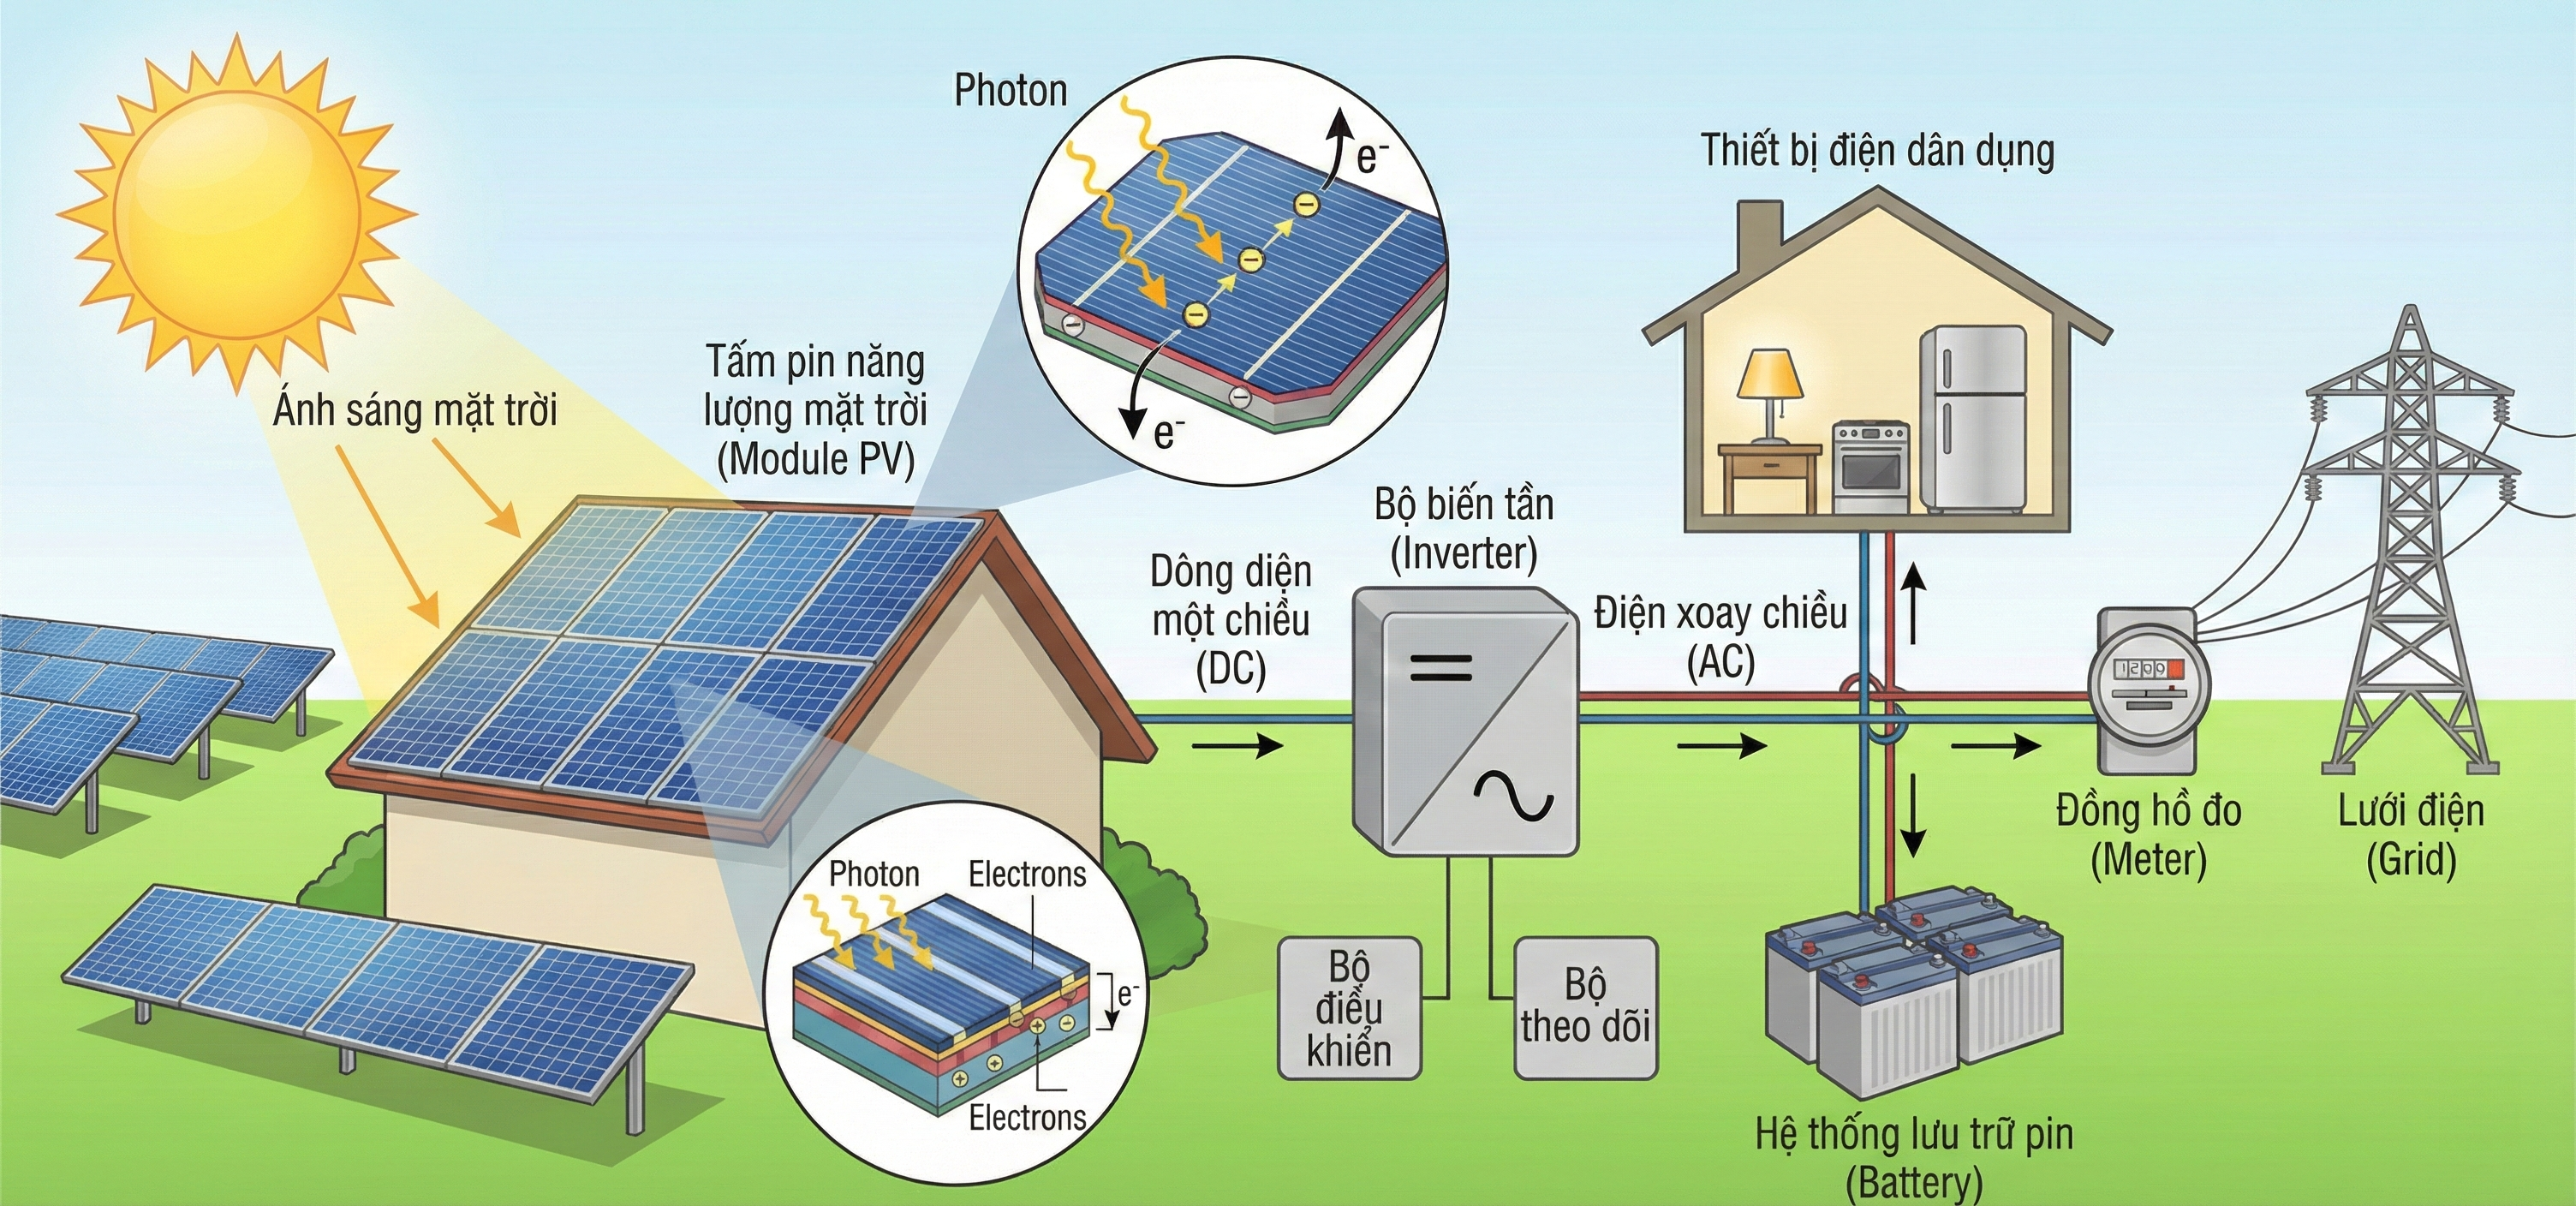
\includegraphics[width=0.8\textwidth]{images/TongQuan/pinmattroi.png}
	\end{center}
\end{frame}

%------------------------------------------------
% SLIDE 10: ẨN - Tổng quan tiềm năng (đã gộp vào slide 11)
% \begin{frame}
% 	\frametitle{TÌNH HÌNH HỆ THỐNG PIN MẶT TRỜI TRÊN THẾ GIỚI}
% 	
% 	\vspace{0.3cm}
% 	
% 	\begin{columns}[t]
% 		% Cột 1: BÙNG NỔ
% 		\begin{column}{0.3\textwidth}
% 			\centering
% 			\includegraphics[width=0.5\textwidth]{images/TongQuan/icons/bungno.png}
% 			
% 			\vspace{0.3cm}
% 			
% 			{\Large\textbf{BÙNG NỔ}}
% 			
% 			\vspace{0.4cm}
% 			
% 			\small
% 			Diện mặt trời chiếm \\
% 			\textcolor{orange}{\textbf{73\%}} tổng công suất \\
% 			năng lượng tái tạo \\
% 			tăng thêm toàn cầu \\
% 			năm 2023.
% 		\end{column}
% 
% 		\vrule width 1pt
% 		
% 		% Cột 2: CHI PHÍ
% 		\begin{column}{0.3\textwidth}
% 			\centering
% 			\includegraphics[width=0.5\textwidth]{images/TongQuan/icons/chiphi.png}
% 			
% 			\vspace{0.3cm}
% 			
% 			{\Large\textbf{CHI PHÍ}}
% 			
% 			\vspace{0.4cm}
% 			
% 			\small
% 			Chi phí lắp đặt đã giảm sâu \\
% 			\textcolor{orange}{\textbf{85\%}} sau một thập kỷ, trở \\
% 			thành nguồn năng lượng \\
% 			dễ tiếp cận nhất.
% 		\end{column}
% 
% 		\vrule width 1pt
% 		
% 		% Cột 3: TIỀM NĂNG
% 		\begin{column}{0.3\textwidth}
% 			\centering
% 			\includegraphics[width=0.5\textwidth]{images/TongQuan/icons/tiemnang.png}
% 			
% 			\vspace{0.3cm}
% 			
% 			{\Large\textbf{TIỀM NĂNG}}
% 			
% 			\vspace{0.4cm}
% 			
% 			\small
% 			Việt Nam nằm trong \\
% 			``vùng đỏ'' bức xạ nhiệt, \\
% 			mang hữu tiềm năng tự \\
% 			nhiên lý tưởng để phát \\
% 			triển điện mặt trời.
% 		\end{column}
% 	\end{columns}
% 	
% \end{frame}

% SLIDE 11: GIỮ LẠI - Biểu đồ tăng trưởng (ấn tượng nhất)


% SLIDE 12: ẨN - Biểu đồ chi phí
% \begin{frame}
% \label{Chiphi}
% 	\frametitle{TÌNH HÌNH HỆ THỐNG PIN MẶT TRỜI TRÊN THẾ GIỚI}
% 	\begin{center}
% 		\includegraphics[width=0.6\textwidth]{images/TongQuan/bieudochiphi.png}
% 	\end{center}
% \end{frame}

% SLIDE 13: ẨN - Bản đồ bức xạ thế giới
% \begin{frame}
% \label{Nhiet}
% 	\frametitle{TÌNH HÌNH HỆ THỐNG PIN MẶT TRỜI TRÊN THẾ GIỚI}
% 	\begin{center}
% 		\includegraphics[width=0.8\textwidth]{images/TongQuan/bieudonhiet.png}
% 	\end{center}
% \end{frame}



% Định nghĩa màu nền xanh
\definecolor{CardBlue}{HTML}{B1CDFC}

\begin{frame}
    \frametitle{TÌNH HÌNH HỆ THỐNG PIN MẶT TRỜI TẠI VIỆT NAM}
    \vspace{-0.85cm}
    
    \begin{columns}[t, onlytextwidth]
        \tcbset{
            mycardstyle/.style={
                colback=white,
                colframe=gray!50,
                arc=6pt,
                boxrule=1pt,
                left=2pt, right=2pt, top=1pt, bottom=1pt,
                equal height group=A,
                fontupper=\scriptsize,
                halign=center,
                valign=top
            }
        }

        % --- Card 1 ---
        \begin{column}{0.31\textwidth}
            \begin{tcolorbox}[mycardstyle]
                \begin{minipage}[t][2.95cm][t]{\linewidth}
                    \raggedright
                    % Tiêu đề
                    \centering
                    {\bfseries\small ĐIỆN MẶT TRỜI\\QUY MÔ LỚN}
                    
                    \vspace{0.15cm}
                    \raggedright
                    \textbullet\ Nguồn cung cấp sản lượng điện lớn đóng góp vào lưới điện quốc gia.\\[0.05cm]
                    \textbullet\ Các dự án kỷ lục: nhà máy Dầu Tiếng, tổ hợp Trung Nam.
                \end{minipage}
                
                % Yêu cầu 2: Ảnh bo góc bằng TikZ Clip
                \begin{tikzpicture}
                    \clip [rounded corners=6pt] (0,0) rectangle (\linewidth, 2.2cm); 
                    \node[anchor=south west, inner sep=0] at (0,0) {\includegraphics[width=\linewidth, height=2.2cm]{images/TongQuan/trungnam.jpg}};
                \end{tikzpicture}
            \end{tcolorbox}
        \end{column}\hfill

        % --- Card 2 ---
        \begin{column}{0.31\textwidth}
            \begin{tcolorbox}[mycardstyle]
                \begin{minipage}[t][2.95cm][t]{\linewidth}
                    \raggedright
                    \centering
                    {\bfseries\small ĐIỆN MẶT TRỜI\\ÁP MÁI}
                    
                    \vspace{0.15cm}
                    \raggedright
                    \textbullet\ Tận dụng mái nhà xưởng và hộ gia đình.\\[0.05cm]
                    \textbullet\ Ưu tiên hàng đầu: không tốn đất, giảm tải tại chỗ cho lưới điện.
                \end{minipage}
                
                \begin{tikzpicture}
                    \clip [rounded corners=6pt] (0,0) rectangle (\linewidth, 2.2cm);
                    \node[anchor=south west, inner sep=0] at (0,0) {\includegraphics[width=\linewidth, height=2.2cm]{images/TongQuan/apmai.png}};
                \end{tikzpicture}
            \end{tcolorbox}
        \end{column}\hfill

        % --- Card 3 ---
        \begin{column}{0.31\textwidth}
            \begin{tcolorbox}[mycardstyle]
                \begin{minipage}[t][2.95cm][t]{\linewidth}
                    \raggedright
                    \centering
                    {\bfseries\small ĐIỆN MẶT TRỜI\\ĐỘC LẬP}
                    
                    \vspace{0.15cm}
                    \raggedright
                    \textbullet\ Khu vực chưa có điện lưới hoặc công trình độc lập.\\[0.05cm]
                    \textbullet\ Cần tính toán kỹ pin lưu trữ để đảm bảo ổn định.
                \end{minipage}
                
                \begin{tikzpicture}
                    \clip [rounded corners=6pt] (0,0) rectangle (\linewidth, 2.2cm);
                    \node[anchor=south west, inner sep=0] at (0,0) {\includegraphics[width=\linewidth, height=2.2cm]{images/TongQuan/doclap.png}};
                \end{tikzpicture}
            \end{tcolorbox}
        \end{column}\hfill
        
    \end{columns}

\end{frame}

% Định nghĩa màu sắc giống trong ảnh
\definecolor{mypaleblue}{RGB}{189, 215, 238} % Màu xanh nhạt cho đường kẻ
\definecolor{myorange}{RGB}{197, 90, 17}    % Màu cam đậm cho tiêu đề (nếu cần)
\definecolor{myblueicon}{RGB}{0, 112, 192}  % Màu xanh cho icon

% --- KHAI BÁO LỆNH BO GÓC BẰNG TIKZ (ĐẶT NGOÀI FRAME) ---
% Nguyên lý: Vẽ 1 ảnh tàng hình để lấy kích thước -> Tạo khung cắt bo tròn -> Vẽ ảnh thật đè lên
\newcommand{\roundimg}[2]{ % Tham số: #1 = chiều cao, #2 = đường dẫn ảnh
    \begin{tikzpicture}[baseline=(img.center)]
        \node[inner sep=0pt, opacity=0] (measure) {\includegraphics[height=#1]{#2}}; % Ảnh tàng hình đo size
        \clip[rounded corners=8pt] (measure.south west) rectangle (measure.north east); % Cắt bo góc
        \node[inner sep=0pt] (img) at (measure.center) {\includegraphics[height=#1]{#2}}; % Ảnh thật
    \end{tikzpicture}
}
% -----------------------------------------------------------------------

\begin{frame}
    \frametitle{CÁC DẠNG HƯ HỎNG PHỔ BIẾN}

    \vspace*{-0.4cm} 
    
    \begin{columns}[T]
        
        % --- CỘT 1 ---
        \begin{column}{0.32\textwidth}
            % GÓI GỌN TEXT VÀO MINIPAGE ĐỂ CỐ ĐỊNH CHIỀU CAO -> ẢNH SẼ THẲNG HÀNG
            \begin{minipage}[t][3.3cm][t]{\linewidth}
                \centering
                \textbf{\large Suy Thoái Quang Học}
                
                \vspace{0.1cm}
                \small \raggedright
                \begin{itemize}
                    \setlength\itemsep{0.02cm}
                    \setlength\parskip{0pt}
                    \item \textbf{Bụi bẩn:} Giảm khả năng hấp thụ ánh sáng.
                    \item \textbf{Ố màu:} Lão hóa vật liệu.
                    \item \textbf{Bong tróc:} Tách lớp kính bảo vệ.
                \end{itemize}
            \end{minipage}
            
            \vspace{0.1cm}
            \centering
            % Chỉnh size ảnh nhỏ lại (1.4cm) để tránh tràn slide
            \begin{tikzpicture}
                \clip [rounded corners=6pt] (0,0) rectangle (3.6cm, 2.0cm);
                \node[inner sep=0pt, anchor=center] at (1.8cm, 1.0cm) {\includegraphics[width=3.6cm, height=2.0cm]{images/TongQuan/suythoaiquanghoc.png}};
            \end{tikzpicture}
        \end{column}

        % --- KẺ DỌC 1 ---
        \begin{column}{0.02\textwidth}
            \centering
            % Điều chỉnh chiều dài thanh kẻ dọc cho vừa vặn
            \raisebox{-0.8cm}{\color{mypaleblue}\rule{1pt}{4.5cm}}
        \end{column}

        % --- CỘT 2 ---
        \begin{column}{0.32\textwidth}
            \begin{minipage}[t][3.3cm][t]{\linewidth}
                \centering
                \textbf{\large Mất Kết Nối Điện}
                
                \vspace{0.1cm}
                \small \raggedright
                \begin{itemize}
                    \setlength\itemsep{0.02cm}
                    \setlength\parskip{0pt}
                    \item \textbf{Vết nứt:} Do tác động cơ học/nhiệt.
                    \item \textbf{Điểm nóng:} Gây quá nhiệt cục bộ.
                    \item \textbf{Ngắn mạch:} Hư hỏng cell pin.
                \end{itemize}
            \end{minipage}

            \vspace{0.1cm}
            \centering
            \begin{tikzpicture}
                \clip [rounded corners=6pt] (0,0) rectangle (3.6cm, 2.0cm);
                \node[inner sep=0pt, anchor=center] at (1.8cm, 1.0cm) {\includegraphics[width=3.6cm, height=2.0cm]{images/TongQuan/matketnoidien.jpg}};
            \end{tikzpicture}
        \end{column}

        % --- KẺ DỌC 2 ---
        \begin{column}{0.02\textwidth}
            \centering
            \raisebox{-0.8cm}{\color{mypaleblue}\rule{1pt}{4.5cm}}
        \end{column}

        % --- CỘT 3 ---
        \begin{column}{0.32\textwidth}
            \begin{minipage}[t][3.3cm][t]{\linewidth}
                \centering
                \textbf{\large Hư Hỏng Phần Cứng}
                
                \vspace{0.1cm}
                \small \raggedright
                \begin{itemize}
                    \setlength\itemsep{0.02cm}
                    \setlength\parskip{0pt}
                    \item \textbf{PID:} Suy giảm do điện thế cảm ứng.
                    \item \textbf{Diode hỏng:} Mất chức năng bypass.
                    \item \textbf{Lỗi dây:} Ăn mòn, đứt gãy.
                \end{itemize}
            \end{minipage}
            
            \vspace{0.1cm}
            \centering
            \begin{tikzpicture}
                \clip [rounded corners=6pt] (0,0) rectangle (3.6cm, 2.0cm);
                \node[inner sep=0pt, anchor=center] at (1.8cm, 1.0cm) {\includegraphics[width=3.6cm, height=2.0cm]{images/TongQuan/huhongphancung.png}};
            \end{tikzpicture}
        \end{column}
    \end{columns}
\end{frame}

\begin{frame}
    \frametitle{GIỚI THIỆU VỀ UAV}

    % --- 1. KÉO SÁT LÊN TRÊN ---
    \vspace{-0.3cm}

    % --- 2. DANH SÁCH ---
    \footnotesize
    \begin{itemize}
        \setlength\itemsep{0pt}
        \setlength\parskip{0pt}
        \item Nhóm chọn giải pháp kiểm tra hệ thống bằng thiết bị bay không người lái (UAV) tích hợp Camera quang học (RGB).
        \item Hướng tiếp cận này khắc phục nhược điểm về chi phí cao và tốn kém nhân lực của các phương pháp truyền thống.
        \item Giải pháp loại bỏ tình trạng quá tải, tốn thời gian và nguy cơ bỏ sót lỗi khi phân tích thủ công lượng lớn hình ảnh.
    \end{itemize}

    \vspace{0.2cm} % Tăng khoảng cách một chút để thoáng hơn

    % --- PHẦN NỘI DUNG CHÍNH ---
    \begin{columns}[T, onlytextwidth]
        % --- CỘT TRÁI: BẢNG ĐÁNH GIÁ ---
        % Giảm độ rộng cột trái một chút để nhường chỗ cho cột phải
        \begin{column}{0.45\textwidth}
            \centering % <--- THÊM LỆNH NÀY ĐỂ CANH GIỮA BẢNG TRONG CỘT (DỊCH PHẢI 1 TÍ)
            \begin{table}[h]
                \scriptsize
                \renewcommand{\arraystretch}{1.2} % Tăng nhẹ giãn dòng cho dễ đọc
                \setlength{\tabcolsep}{3pt}
                % Sử dụng tỷ lệ phần trăm để bảng tự co giãn tốt hơn
                \begin{tabular}{|p{0.25\linewidth}|p{0.68\linewidth}|}
                    \hline
                    \rowcolor{blue!70}\textcolor{white}{\textbf{Đánh giá}} & \cellcolor{blue!70} \\
                    \hline
                    \cellcolor{green!20}\textbf{Ưu điểm} & Tối ưu chi phí, tốc độ; giảm tải nhân lực, dễ triển khai. \\
                    \hline
                    \cellcolor{red!20}\textbf{Hạn chế} & Chỉ phát hiện lỗi bề mặt; độ chính xác phụ thuộc đk bay. \\
                    \hline
                \end{tabular}
            \end{table}
        \end{column}

        % --- CỘT PHẢI: SƠ ĐỒ QUY TRÌNH MỚI ---
        % Tăng độ rộng cột phải để chứa sơ đồ lớn hơn
        \begin{column}{0.53\textwidth}
            \centering
            % Sử dụng resizebox để ép toàn bộ sơ đồ vừa khít chiều ngang cột
            \resizebox{1\linewidth}{!}{%
                \begin{tikzpicture}[
                    % Định nghĩa kiểu cho các hộp và nhãn
                    boxstyle/.style={
                        draw,
                        rectangle,
                        fill=blue!15, % Màu nền xanh nhạt giống ảnh
                        align=center,
                        font=\bfseries\small, % Chữ in đậm, to vừa
                        text width=3.2cm, % Độ rộng cố định cho các hộp
                        minimum height=1.2cm,
                        inner sep=5pt
                    },
                    labelstyle/.style={
                        align=center,
                        font=\scriptsize, % Chữ chú thích nhỏ hơn
                        text width=3.2cm,
                        below=0.2cm % Khoảng cách nằm dưới hộp
                    },
                    arrowstyle/.style={->, >=latex, thick} % Kiểu mũi tên
                ]

                    % 1. Node Drone ở trên cùng, giữa
                    % Thay đường dẫn ảnh bằng ảnh thực tế của bạn: images/TongQuan/drone.png
                    \node (drone) at (0, 3) {\includegraphics[width=2.5cm, keepaspectratio]{images/TongQuan/drone.png}};

                    % 2. Các hộp quy trình chính (Đặt hộp số 2 ở giữa tâm 0,0)
                    \node [boxstyle] (step2) at (0,0) {2. Thu thập dữ liệu RGB};
                    % Hộp 1 nằm bên trái hộp 2
                    \node [boxstyle, left=0.6cm of step2] (step1) {1. Lập kế hoạch bay};
                    % Hộp 3 nằm bên phải hộp 2
                    \node [boxstyle, right=0.6cm of step2] (step3) {3. AI Detect (Deep Learning)};

                    % 3. Các nhãn chú thích bên dưới các hộp
                    \node [labelstyle] at (step1.south) {Thiết lập đường bay tự động};
                    \node [labelstyle] at (step2.south) {Chụp ảnh, gắn thẻ GPS, ghép bản đồ};
                    \node [labelstyle] at (step3.south) {Phân tích lỗi \& Định vị tọa độ};

                    % 4. Các mũi tên kết nối
                    % Mũi tên nét đứt từ Drone xuống hộp 2
                    \draw [arrowstyle, dashed, very thick, gray!80] (drone.south) -- (step2.north);
                    % Mũi tên từ 1 sang 2
                    \draw [arrowstyle] (step1) -- (step2);
                    % Mũi tên từ 2 sang 3
                    \draw [arrowstyle] (step2) -- (step3);

                \end{tikzpicture}
            }% Kết thúc resizebox
        \end{column}
    \end{columns}
\end{frame}

\begin{frame}[t]
    \frametitle{CÁC PHƯƠNG PHÁP KIỂM TRA \& ĐÁNH GIÁ KHÁC}
    \vspace{-0.3cm}
    
    \begin{columns}[T, onlytextwidth]
        % --- CỘT 1: MẮT THƯỜNG ---
        \begin{column}{0.24\textwidth}
            \centering
            {\bfseries\small\textcolor{black}{MẮT THƯỜNG\strut}}\par
            \vspace{0.1cm}
            \begin{tikzpicture}
                % Ảnh ảo để lấy kích thước khung (height=2.2cm)
                \node[inner sep=0pt, opacity=0] (measure) {\includegraphics[width=\linewidth, height=2.2cm, keepaspectratio=false]{\pathImages visual_inspection_worker.png}};
                % Cắt ảnh thật
                \begin{scope}
                    \clip[rounded corners=10pt] (measure.south west) rectangle (measure.north east);
                    \node[inner sep=0pt] at (measure.center) {\includegraphics[width=\linewidth, height=2.2cm, keepaspectratio=false]{\pathImages visual_inspection_worker.png}};
                \end{scope}
            \end{tikzpicture}
            \vspace{0.05cm}
            \scriptsize \raggedright
            \begin{itemize}
                \setlength\itemsep{0pt} \setlength\parskip{0pt} \setlength\leftmargini{0.3cm}
                \item Sàng lọc lỗi bề mặt (kính, khung).
                \item Chi phí thấp.
            \end{itemize}
        \end{column}\hfill
        % --- CỘT 2: ĐIỆN HỌC (Zoom to hơn) ---
        \begin{column}{0.24\textwidth}
            \centering
            {\bfseries\small\textcolor{black}{ĐIỆN HỌC\strut}}\par
            \vspace{0.1cm}
            \begin{tikzpicture}
                \node[inner sep=0pt, opacity=0] (measure) {\includegraphics[width=\linewidth, height=2.2cm, keepaspectratio=false]{\pathImages iv_curve_device.png}};
                \begin{scope}
                    \clip[rounded corners=10pt] (measure.south west) rectangle (measure.north east);
                    % Zoom ảnh lên 1.4 lần (2.2 * 1.4 = 3.08cm)
                    \node[inner sep=0pt] at (measure.center) {\includegraphics[width=1.4\linewidth, height=3.08cm, keepaspectratio=false]{\pathImages iv_curve_device.png}};
                \end{scope}
            \end{tikzpicture}
            \vspace{0.05cm}
            \scriptsize \raggedright
            \begin{itemize}
                \setlength\itemsep{0pt} \setlength\parskip{0pt} \setlength\leftmargini{0.3cm}
                \item Đo đường cong I-V.
                \item Kiểm tra sức khỏe dòng điện.
                \item Đánh giá hiệu suất thực tế.
            \end{itemize}
        \end{column}\hfill
        % --- CỘT 3: HÌNH ẢNH ---
        \begin{column}{0.24\textwidth}
            \centering
            {\bfseries\small\textcolor{black}{HÌNH ẢNH\strut}}\par
            \vspace{0.1cm}
            \begin{tikzpicture}
                \node[inner sep=0pt, opacity=0] (measure) {\includegraphics[width=\linewidth, height=2.2cm, keepaspectratio=false]{\pathImages el_images.png}};
                \begin{scope}
                    \clip[rounded corners=10pt] (measure.south west) rectangle (measure.north east);
                    \node[inner sep=0pt] at (measure.center) {\includegraphics[width=\linewidth, height=2.2cm, keepaspectratio=false]{\pathImages el_images.png}};
                \end{scope}
            \end{tikzpicture}
            \vspace{0.05cm}
            \scriptsize \raggedright
            \begin{itemize}
                \setlength\itemsep{0pt} \setlength\parskip{0pt} \setlength\leftmargini{0.3cm}
                \item \textbf{EL:} Soi xuyên thấu vết nứt.
                \item \textbf{UV-F:} Đánh giá mức độ lão hóa vật liệu.
            \end{itemize}
        \end{column}\hfill
        % --- CỘT 4: VẬT LIỆU ---
        \begin{column}{0.24\textwidth}
            \centering
            {\bfseries\small\textcolor{black}{VẬT LIỆU\strut}}\par
            \vspace{0.1cm}
            \begin{tikzpicture}
                \node[inner sep=0pt, opacity=0] (measure) {\includegraphics[width=\linewidth, height=2.2cm, keepaspectratio=false]{\pathImages spectrometer_lab.png}};
                \begin{scope}
                    \clip[rounded corners=10pt] (measure.south west) rectangle (measure.north east);
                    \node[inner sep=0pt] at (measure.center) {\includegraphics[width=\linewidth, height=2.2cm, keepaspectratio=false]{\pathImages spectrometer_lab.png}};
                \end{scope}
            \end{tikzpicture}
            \vspace{0.05cm}
            \scriptsize \raggedright
            \begin{itemize}
                \setlength\itemsep{0pt} \setlength\parskip{0pt} \setlength\leftmargini{0.3cm}
                \item Phân tích quang phổ chuyên sâu.
                \item Kiểm tra cấu trúc trong phòng Lab.
            \end{itemize}
        \end{column}
    \end{columns}

\end{frame}

\begin{frame}
    \frametitle{TỔNG HỢP \& SO SÁNH CÁC PHƯƠNG PHÁP}
    \definecolor{headerBlue}{HTML}{6FA8DC}
    
    % Kéo bảng lên sát mép trên hơn nữa (từ -0.5cm lên -0.65cm)
    \vspace{-0.65cm} 
    
    \begin{table}
        \centering
        \resizebox{\textwidth}{!}{
            % Giữ nguyên scriptsize như bạn muốn (không dùng tiny)
            \scriptsize 
            
            % Giảm giãn dòng xuống 0.75 (Vẫn đọc tốt, tiết kiệm chiều cao cực nhiều)
            \setlength{\tabcolsep}{3pt} 
            \renewcommand{\arraystretch}{0.75} 
            
            \begin{tabular}{|
                >{\raggedright\arraybackslash}p{2.2cm}|
                >{\raggedright\arraybackslash}p{5.5cm}|
                >{\raggedright\arraybackslash}p{4.0cm}|
                >{\raggedright\arraybackslash}p{6.0cm}|
            }
                \hline
                \rowcolor{headerBlue} 
                \textbf{Công nghệ} & \textbf{Đầu vào} & \textbf{Phương pháp} & \textbf{Kết quả} \\
                \hline
                
                % Hàng 1
                Chụp ảnh đa phổ & 
                - Ảnh không lỗi: 15330 \newline - Ảnh lỗi: 5915 \newline - Train/Test: 80/20 & 
                Mạng neural tích chập đa phổ & 
                Độ chính xác: \newline - Đường kẻ dày: 76.4\% \newline - Vết xước: 48.6\% \newline - Tế bào bẩn: 87.2\% \\
                \hline
                
                % Hàng 2
                Chụp ảnh nhiệt hồng ngoại (IR) & 
                18 video: \newline - 13 (72\%) huấn luyện \newline - 5 (28\%) kiểm thử & 
                - YOLOv2 \newline - YOLOv3 & 
                - YOLOv2: Accuracy 89\% \newline - YOLOv3: Accuracy 91\% \\
                \hline
                
                % Hàng 3
                Chụp ảnh RGB & 
                - Dữ liệu gốc: 45754 \newline - Huấn luyện: 27537 \newline - Xác thực: 18217 & 
                - ImpactNet \newline - Mask FCNN \newline - BiDAF \newline - WebNN & 
                Bụi, Tuyết, Phân chim, Vết nứt với độ chính xác tổng thể là 84.5\% \\
                \hline
                
                % Hàng 4: Đã viết gọn tên công nghệ để tránh xuống dòng quá nhiều
                Camera CCD, Nhiệt (IR) \& RGB & 
                Ảnh từ UAV: \newline 
                + 2038 ảnh nhiệt: Train 1426, Test 306, Val 306 \newline
                + 1500 ảnh KTS: Train 1050, Test 225, Val 225 & 
                - Biến đổi hình thái \& Canny \newline 
                - Xử lý ảnh nhiệt \& CCD \newline 
                - Biến đổi Hough \newline 
                - Xoay ảnh, YOLOv3 & 
                Độ chính xác tổng thể 92\% (Điểm nóng, vết nứt...). \newline
                Chi tiết: \newline 
                - Điểm nóng: 80.3\% \newline
                - Dính hộp nối: 90.2\% \newline
                - Vũng nước: 82.5\% \\
                \hline
                
                % Hàng 5: Viết gọn tên công nghệ
                Ảnh phát quang hồng ngoại gần & 
                Tập dữ liệu chuẩn PVEL-AD-2021 & 
                YOLOv7 & 
                Precision: 88.3\% \\
                \hline
                
                % Hàng 6
                Chụp ảnh điện quang EL & 
                148 ảnh tế bào quang điện (U-net): \newline - Train: 108 (73\%) \newline - Test: 30 (20\%) \newline - Val: 10 (7\%) & 
                - VGG-16 \newline - U-net & 
                Recall: \newline - Vết nứt: 84\% \newline - Vùng k.hoạt động: 69\% \newline - Lỗi đường dẫn pin: 53\% \\
                \hline
            \end{tabular}
        }
    \end{table}
\end{frame}

\begin{frame}
    \frametitle{MÔ HÌNH EfficientNet-B2}

    % [QUAN TRỌNG] Sử dụng shrink để tự động co giãn nếu vẫn bị tràn chút ít (tùy chọn)
    % Hoặc bỏ [shrink] nếu code bên dưới đã vừa vặn.
    
    \begin{columns}[T] 
        
        % --- CỘT TRÁI: VĂN BẢN ---
        \begin{column}{0.6\textwidth} % Tăng độ rộng cột chữ lên một chút cho thoáng
            
            % Dùng \footnotesize thay vì \small để chữ nhỏ hơn, vừa trang
            \footnotesize 
            
            % Tiêu đề
            {\textbf{\textcolor{red}{Tại sao chọn EfficientNet-B2 ?}}}
            \vspace{0.1cm} % Giảm khoảng cách (từ 0.3 xuống 0.1)

            % Nội dung
            Kiến trúc này sử dụng phương pháp \textbf{Compound Scaling}, cân bằng tối ưu giữa 3 yếu tố: độ sâu (depth), độ rộng (width) và độ phân giải (resolution).
            \vspace{0.1cm} % Giảm khoảng cách

            % Danh sách
            \begin{itemize}
                % Giảm khoảng cách giữa các item (từ 0.8em xuống 0.3em)
                \setlength\itemsep{0.3em} 
                
                \item[\textcolor{cyan}{\checkmark}] \textbf{Số lượng tham số:} 7.7 Triệu.
                
                \item[\textcolor{cyan}{\checkmark}] \textbf{Khối MBConv:} Mobile Inverted Bottleneck giúp giảm chi phí tính toán.
                
                \item[\textcolor{cyan}{\checkmark}] \textbf{Squeeze-and-Excitation (SE):} Cơ chế Attention giúp tập trung đặc trưng lỗi.
                
                \item[\textcolor{cyan}{\checkmark}] \textbf{Transfer Learning:} Dùng trọng số ImageNet để hội tụ nhanh.
            \end{itemize}

            \vspace{0.2cm} % Giảm khoảng cách cuối
            \textbf{Hàm mất mát (Loss Function):} Kết hợp Weighted Cross-Entropy và Focal Loss
        \end{column}

        % --- CỘT PHẢI: HÌNH ẢNH ---
        \begin{column}{0.4\textwidth}
            \centering
            % Giảm chiều cao ảnh xuống 75% chiều cao slide (thay vì 0.8) để tránh đẩy khung
            \includegraphics[width=\textwidth, height=0.75\textheight, keepaspectratio]{images/TongQuan/mohinhe2.png}
        \end{column}

    \end{columns}
\end{frame}

% Định nghĩa màu sắc
\definecolor{myRed}{HTML}{FF3333}
\definecolor{bgGray}{HTML}{F8FAFC}
\definecolor{textDark}{HTML}{333333}
\begin{frame}
    \frametitle{ĐÁNH GIÁ MÔ HÌNH}

    % Tiêu đề chính
    \begin{center}
        \textbf{\textcolor{myRed}{\large Tại Sao Cần Đánh Giá Mô Hình?}}
    \end{center}
    
    \vspace{0.2cm} % Giảm khoảng cách để tránh tràn trang

    % Chia 2 cột lớn độc lập cho toàn bộ slide
    \begin{columns}[T] % T = Top alignment (căn đỉnh trên)
        
        % --- CỘT TRÁI: Khả năng tổng quát hóa ---
        \begin{column}{0.48\textwidth}
            \begin{tcolorbox}[
                enhanced, equal height group=evalbox,
                colback=bgGray,
                colframe=bgGray,
                arc=8pt,
                boxrule=0pt,
                left=4pt, right=4pt, top=6pt, bottom=6pt
            ]
                % Chia cột nhỏ bên trong Box (Icon | Tiêu đề)
                \begin{columns}
                    % Cột chứa Icon (nhỏ lại theo yêu cầu)
                    \begin{column}{0.15\textwidth}
                        \centering
                        % Đặt kích thước cố định nhỏ (0.8cm)
                        \includegraphics[width=0.6cm, keepaspectratio]{images/TongQuan/icons/khaiquat.png}
                    \end{column}
                    % Cột chứa Tiêu đề
                    \begin{column}{0.83\textwidth}
                        \textbf{\small Khả năng tổng quát hóa}
                    \end{column}
                \end{columns}

                \vspace{0.2cm}
                
                % Nội dung text
                \justifying
                \color{textDark}
                \footnotesize % Dùng font nhỏ hơn một chút để an toàn
                Mục tiêu cuối cùng không chỉ là khớp dữ liệu huấn luyện (Training Data) mà là hoạt động tốt trên dữ liệu chưa biết (Unseen Data).
            \end{tcolorbox}
        \end{column}

        % --- CỘT PHẢI: Overfitting vs Underfitting ---
        \begin{column}{0.48\textwidth}
            \begin{tcolorbox}[
                enhanced, equal height group=evalbox,
                colback=bgGray,
                colframe=bgGray,
                arc=8pt,
                boxrule=0pt,
                left=4pt, right=4pt, top=6pt, bottom=6pt
            ]
                % Chia cột nhỏ bên trong Box
                \begin{columns}
                    \begin{column}{0.15\textwidth}
                        \centering
                        \includegraphics[width=0.8cm, keepaspectratio]{images/TongQuan/icons/over.png}
                    \end{column}
                    \begin{column}{0.83\textwidth}
                        \textbf{\small Overfitting vs Underfitting}
                    \end{column}
                \end{columns}

                \vspace{0.2cm}

                % Nội dung text
                \justifying
                \color{textDark}
                \footnotesize
                Cân bằng giữa Bias và Variance. Tránh Overfitting (học nhiễu) và Underfitting (chưa bắt được quy luật) để tối ưu hóa hiệu suất thực tế.
            \end{tcolorbox}
        \end{column}

    \end{columns}

\end{frame}

% Định nghĩa màu (giữ nguyên)
\definecolor{mygreen}{RGB}{0, 168, 89} 
\definecolor{myred}{RGB}{237, 28, 36}

\begin{frame}
    \frametitle{MA TRẬN NHẦM LẪN}

    % Thêm [T] để căn nội dung bắt đầu từ trên cùng của cột
    \begin{columns}[T] 
        
        % Cột bên trái: Nội dung văn bản
        \begin{column}{0.55\textwidth}
            \small % Cỡ chữ nhỏ
            Là nền tảng của hầu hết các chỉ số đánh giá phân loại. Nó so sánh kết quả dự đoán với thực tế.
            \vspace{0.1cm} % GIẢM khoảng cách ở đây (từ 0.3 xuống 0.1)

            \begin{itemize}
                % GIẢM khoảng cách giữa các gạch đầu dòng (từ 0.5em xuống 0.1em)
                \setlength\itemsep{0.1em} 
                \setlength\parskip{0pt} % Loại bỏ khoảng cách đoạn thừa
                
                \item \textbf{\textcolor{mygreen}{TP (True Positive):}} Dự đoán đúng là Dương tính.
                
                \item \textbf{\textcolor{mygreen}{TN (True Negative):}} Dự đoán đúng là Âm tính.
                
                \item \textbf{\textcolor{myred}{FP (False Positive):}} Dự đoán sai là Dương tính (Báo động giả).
                
                \item \textbf{\textcolor{myred}{FN (False Negative):}} Dự đoán sai là Âm tính (Bỏ sót).
            \end{itemize}
        \end{column}

        % Cột bên phải: Hình ảnh
        \begin{column}{0.45\textwidth}
            \centering
            % Dùng keepaspectratio để ảnh không bị méo nếu lỡ quá cao
            \includegraphics[width=\textwidth, height=0.7\textheight, keepaspectratio]{images/TongQuan/matran.png}
        \end{column}
    \end{columns}

\end{frame}

% --- ĐỊNH NGHĨA MÀU SẮC ---
\definecolor{myBlueText}{HTML}{155FA0}
\definecolor{myBlueIconBg}{HTML}{E8F0FE}
\definecolor{myBoxBg}{HTML}{F2F6FC}
\definecolor{myBorder}{HTML}{DDDDDD}

% --- MACRO SIÊU GỌN (ULTRA COMPACT) ---
% Đã loại bỏ hết padding thừa để xử lý lỗi 127pt too high
\newcommand{\MetricCard}[4]{
    \begin{tcolorbox}[
        colback=white,
        colframe=myBorder,
        boxrule=1pt,
        arc=6pt,
        width=\linewidth,
        boxsep=0pt, 
        left=2pt, right=2pt, top=1pt, bottom=5pt, 
        before skip=0pt, after skip=0pt, 
        shadow={0.5mm}{-0.5mm}{0mm}{black!5}
    ]
        \centering
        % 1. Header: Icon + Title inline
        \raisebox{-0.22cm}{
            \begin{tikzpicture}
                \node[circle, fill=myBlueIconBg, inner sep=1pt] {
                    \includegraphics[width=0.4cm, height=0.4cm, keepaspectratio]{#1}
                };
            \end{tikzpicture}
        }
        \hspace{0.1cm}
        {\color{myBlueText}\bfseries\small #2} 
        
        \vspace{1pt}

        % 3. Mô tả 
        {\tiny #3}
        \vspace{2pt}

        % 4. Khung công thức
        \begin{tcolorbox}[
            before skip=0pt, after skip=0pt,
            colback=myBoxBg,
            colframe=myBoxBg,
            arc=3pt,
            boxrule=0pt,
            width=0.98\linewidth,
            boxsep=0pt,
            top=2pt, bottom=3pt, left=1pt, right=1pt
        ]
            \centering \color{myBlueText}\bfseries \normalsize
            #4
        \end{tcolorbox}
    \end{tcolorbox}
}

% --- SỬ DỤNG SHRINK=5 NẾU CẦN THIẾT ---
% --- BỎ SHRINK ĐỂ TRÁNH LỖI ARITHMETIC OVERFLOW ---
\begin{frame}
    \frametitle{CHỈ SỐ ĐÁNH GIÁ}
    
    % Kéo nội dung lên sát tiêu đề
    \vspace{-0.3cm} 
    
    \begin{columns}[t]
        % --- CỘT TRÁI ---
        \begin{column}{0.48\textwidth}
            % Accuracy
            \MetricCard%
                {images/TongQuan/icons/chiso/accuracy.png}%
                {Accuracy}%
                {Tỷ lệ dự đoán đúng trên tổng số mẫu.}%
                {$\displaystyle\dfrac{TP+TN}{TP+TN+FP+FN}$}
            
            \vspace{0.15cm} % Khoảng cách giữa 2 thẻ (giữ nhỏ để vừa trang)
            
            % Precision (Nam châm)
            \MetricCard%
                {images/TongQuan/icons/chiso/precision.png}%
                {Precision}%
                {Tỷ lệ phát hiện được dương tính thực tế.}%
                {$\displaystyle\dfrac{TP}{TP+FP}$}
        \end{column}
        
        % --- CỘT PHẢI ---
        \begin{column}{0.48\textwidth}
            % Precision (Phễu)
            \MetricCard%
                {images/TongQuan/icons/chiso/precision2.png}%
                {Recall}%
                {Độ chính xác trong các dự đoán dương tính.}%
                {$\displaystyle\dfrac{TP}{TP+FN}$}
            
            \vspace{0.15cm}
            
            % F1-Score
            \MetricCard%
                {images/TongQuan/icons/chiso/f1score.png}%
                {F1-Score}%
                {Dung hòa Precision \& Recall (data lệch).}%
                {$2 \times \dfrac{P \times R}{P + R}$} 
        \end{column}
    \end{columns}

\end{frame}

%------------------------------------------------
\section{Phương pháp đề xuất}
\SectionIntro{Phần 3: Phương pháp đề xuất}{Quy trình xử lý dữ liệu và kiến trúc mô hình huấn luyện.}
% Định nghĩa màu sắc theo ảnh
\definecolor{processBlue}{RGB}{0, 85, 165}  % Màu xanh đậm của tiêu đề/nút
\definecolor{processRed}{RGB}{235, 50, 50}   % Màu đỏ của số 95%
\definecolor{bgGray}{RGB}{240, 244, 248}     % Màu nền xám nhạt khung dưới
\definecolor{lineGray}{RGB}{200, 200, 200}   % Màu đường kẻ ngang
\begin{frame}
    \frametitle{QUY TRÌNH TỔNG THỂ}

    % 1. Phần mô tả phía trên
    \centering
    \small{Hệ thống được thiết kế khép kín từ khâu thu thập dữ liệu thô đến khi xuất báo cáo phân loại.}
    
    \vspace{0.5cm}

    % 2. Phần sơ đồ Quy trình (Dùng TikZ để căn chỉnh chính xác)
    % resizebox giúp tự động co giãn sơ đồ vừa khít chiều ngang slide, tránh bị tràn
    \resizebox{\textwidth}{!}{
        \begin{tikzpicture}
            % --- Cấu hình khoảng cách ---
            \def\hdist{4.5} % Khoảng cách giữa các bước
            
            % --- Đường kẻ ngang nền ---
            % Vẽ từ tâm icon 1 đến tâm icon 4
            \draw[lineGray, line width=4pt] (0,0) -- ({3*\hdist},0);

            % --- BƯỚC 1: THU THẬP ---
            \node[inner sep=0pt] (icon1) at (0, 1.8) {
                \includegraphics[height=1.5cm]{images/PhuongPhap/icons/camera.png}
            };
            \fill[processBlue] (0,0) circle (6pt); % Chấm tròn xanh
            \node[text width=4cm, align=center, anchor=north] at (0, -0.5) {
                \textbf{\color{processBlue}\large Thu thập} \\[-2pt]
                \small Bay chụp ảnh toàn cảnh \\ bằng UAV
            };

            % --- BƯỚC 2: TIỀN XỬ LÝ ---
            \node[inner sep=0pt] (icon2) at (\hdist, 1.8) {
                \includegraphics[height=1.5cm]{images/PhuongPhap/icons/xulyanh.png}
            };
            \fill[processBlue] (\hdist,0) circle (6pt);
            \node[text width=4cm, align=center, anchor=north] at (\hdist, -0.5) {
                \textbf{\color{processBlue}\large Tiền xử lý} \\[-2pt]
                \small Cắt tách tấm pin \& \\ Chuẩn hóa
            };

            % --- BƯỚC 3: HUẤN LUYỆN ---
            \node[inner sep=0pt] (icon3) at ({2*\hdist}, 1.8) {
                \includegraphics[height=1.5cm]{images/PhuongPhap/icons/train.png}
            };
            \fill[processBlue] ({2*\hdist},0) circle (6pt);
            \node[text width=4cm, align=center, anchor=north] at ({2*\hdist}, -0.5) {
                \textbf{\color{processBlue}\large Huấn luyện} \\[-2pt]
                \small Transfer Learning \\ với EfficientNet-B2
            };

            % --- BƯỚC 4: PHÂN LOẠI ---
            \node[inner sep=0pt] (icon4) at ({3*\hdist}, 1.8) {
                \includegraphics[height=1.5cm]{images/PhuongPhap/icons/classify.png}
            };
            \fill[processBlue] ({3*\hdist},0) circle (6pt);
            \node[text width=4cm, align=center, anchor=north] at ({3*\hdist}, -0.5) {
                \textbf{\color{processBlue}\large Phân loại} \\[-2pt]
                \small Dự đoán nhãn \\ Normal / Defect
            };
        \end{tikzpicture}
    }

    \vspace{0.8cm}

    % 3. Khung Mục tiêu phía dưới
    \begin{tikzpicture}
        \node[
            fill=bgGray, 
            rounded corners=5pt, 
            text width=0.95\textwidth, 
            inner sep=10pt, 
            align=center
        ] {
            \textbf{Mục tiêu:} Tự động hóa hoàn toàn việc phát hiện lỗi bề mặt với độ chính xác \textbf{\color{processRed}>95\%}.
        };
    \end{tikzpicture}

\end{frame}

% Định nghĩa màu
\definecolor{bglight}{HTML}{F2F7FB}
\definecolor{darkblue}{HTML}{0D2B46}
\definecolor{borderblue}{HTML}{2F5575}

% Thêm tùy chọn shrink=5 để tự động co nhỏ 5% nếu vẫn còn hơi chật
\begin{frame}[shrink=5] 
    \frametitle{THU THẬP DỮ LIỆU UAV}

    \begin{columns}[T]
        
        % --- CỘT TRÁI ---
        \begin{column}{0.58\textwidth}
            % Bỏ nền xanh, bỏ viền, đưa padding về 0 để tiết kiệm không gian
            \begin{tcolorbox}[
                enhanced,
                frame hidden,
                colback=white,
                arc=0pt,
                boxrule=0pt,
                left=0pt, right=0pt, top=0pt, bottom=0pt, 
                boxsep=0pt
            ]
                % --- Phần 1: Thiết bị ---
                \textbf{\normalsize Thiết bị} 
                
                \small{DJI Phantom 4 RTK với cảm biến 20MP và công nghệ định vị RTK độ chính xác centimet.}
                
                \vspace{2pt} % Giảm khoảng cách
                
                % --- Phần 2: Thông số ---
                \textbf{\normalsize Thông số bay tối ưu}
                \vspace{1pt}
                
                \begin{itemize}
                     \setlength\itemsep{2pt} % Giảm khoảng cách giữa các item
                     \small 
                     \item[{\includegraphics[height=1em]{images/PhuongPhap/icons/docao.png}}] \textbf{Độ cao:} 25m so với mặt đất.
                     \item[{\includegraphics[height=1em]{images/PhuongPhap/icons/gocchup.png}}] \textbf{Góc chụp:} Vuông góc ($\approx 90^\circ$).
                     \item[{\includegraphics[height=1em]{images/PhuongPhap/icons/thoigian.png}}] \textbf{Thời gian:} 9:00 - 11:00 sáng.
                \end{itemize}

                \vspace{3pt}

                % --- Phần 3: Kết quả ---
                \begin{tcolorbox}[
                    enhanced,
                    title=Kết quả,
                    coltitle=white,
                    fonttitle=\bfseries\small, 
                    colback=bglight,
                    colframe=borderblue,
                    attach boxed title to top left={xshift=0mm, yshift*=-2mm}, 
                    boxed title style={colback=borderblue, sharp corners, rounded corners=southeast, arc=3pt, size=small}, 
                    boxrule=0.5pt,
                    arc=3pt,
                    left=2mm, right=2mm, top=6pt, bottom=2mm, 
                    boxsep=1pt
                ]
                    \small 130 ảnh quang học độ phân giải cao, sắc nét, có tọa độ chính xác.
                \end{tcolorbox}
            \end{tcolorbox}
        \end{column}

        % --- CỘT PHẢI ---
        \begin{column}{0.40\textwidth}
             % Điều chỉnh ảnh bên phải cho khớp chiều cao mới
            \begin{tikzpicture}
                \clip [rounded corners=5pt] (0,0) rectangle (\linewidth, 0.60\paperheight); 
                \node [anchor=south west, inner sep=0] (image) at (0,0) {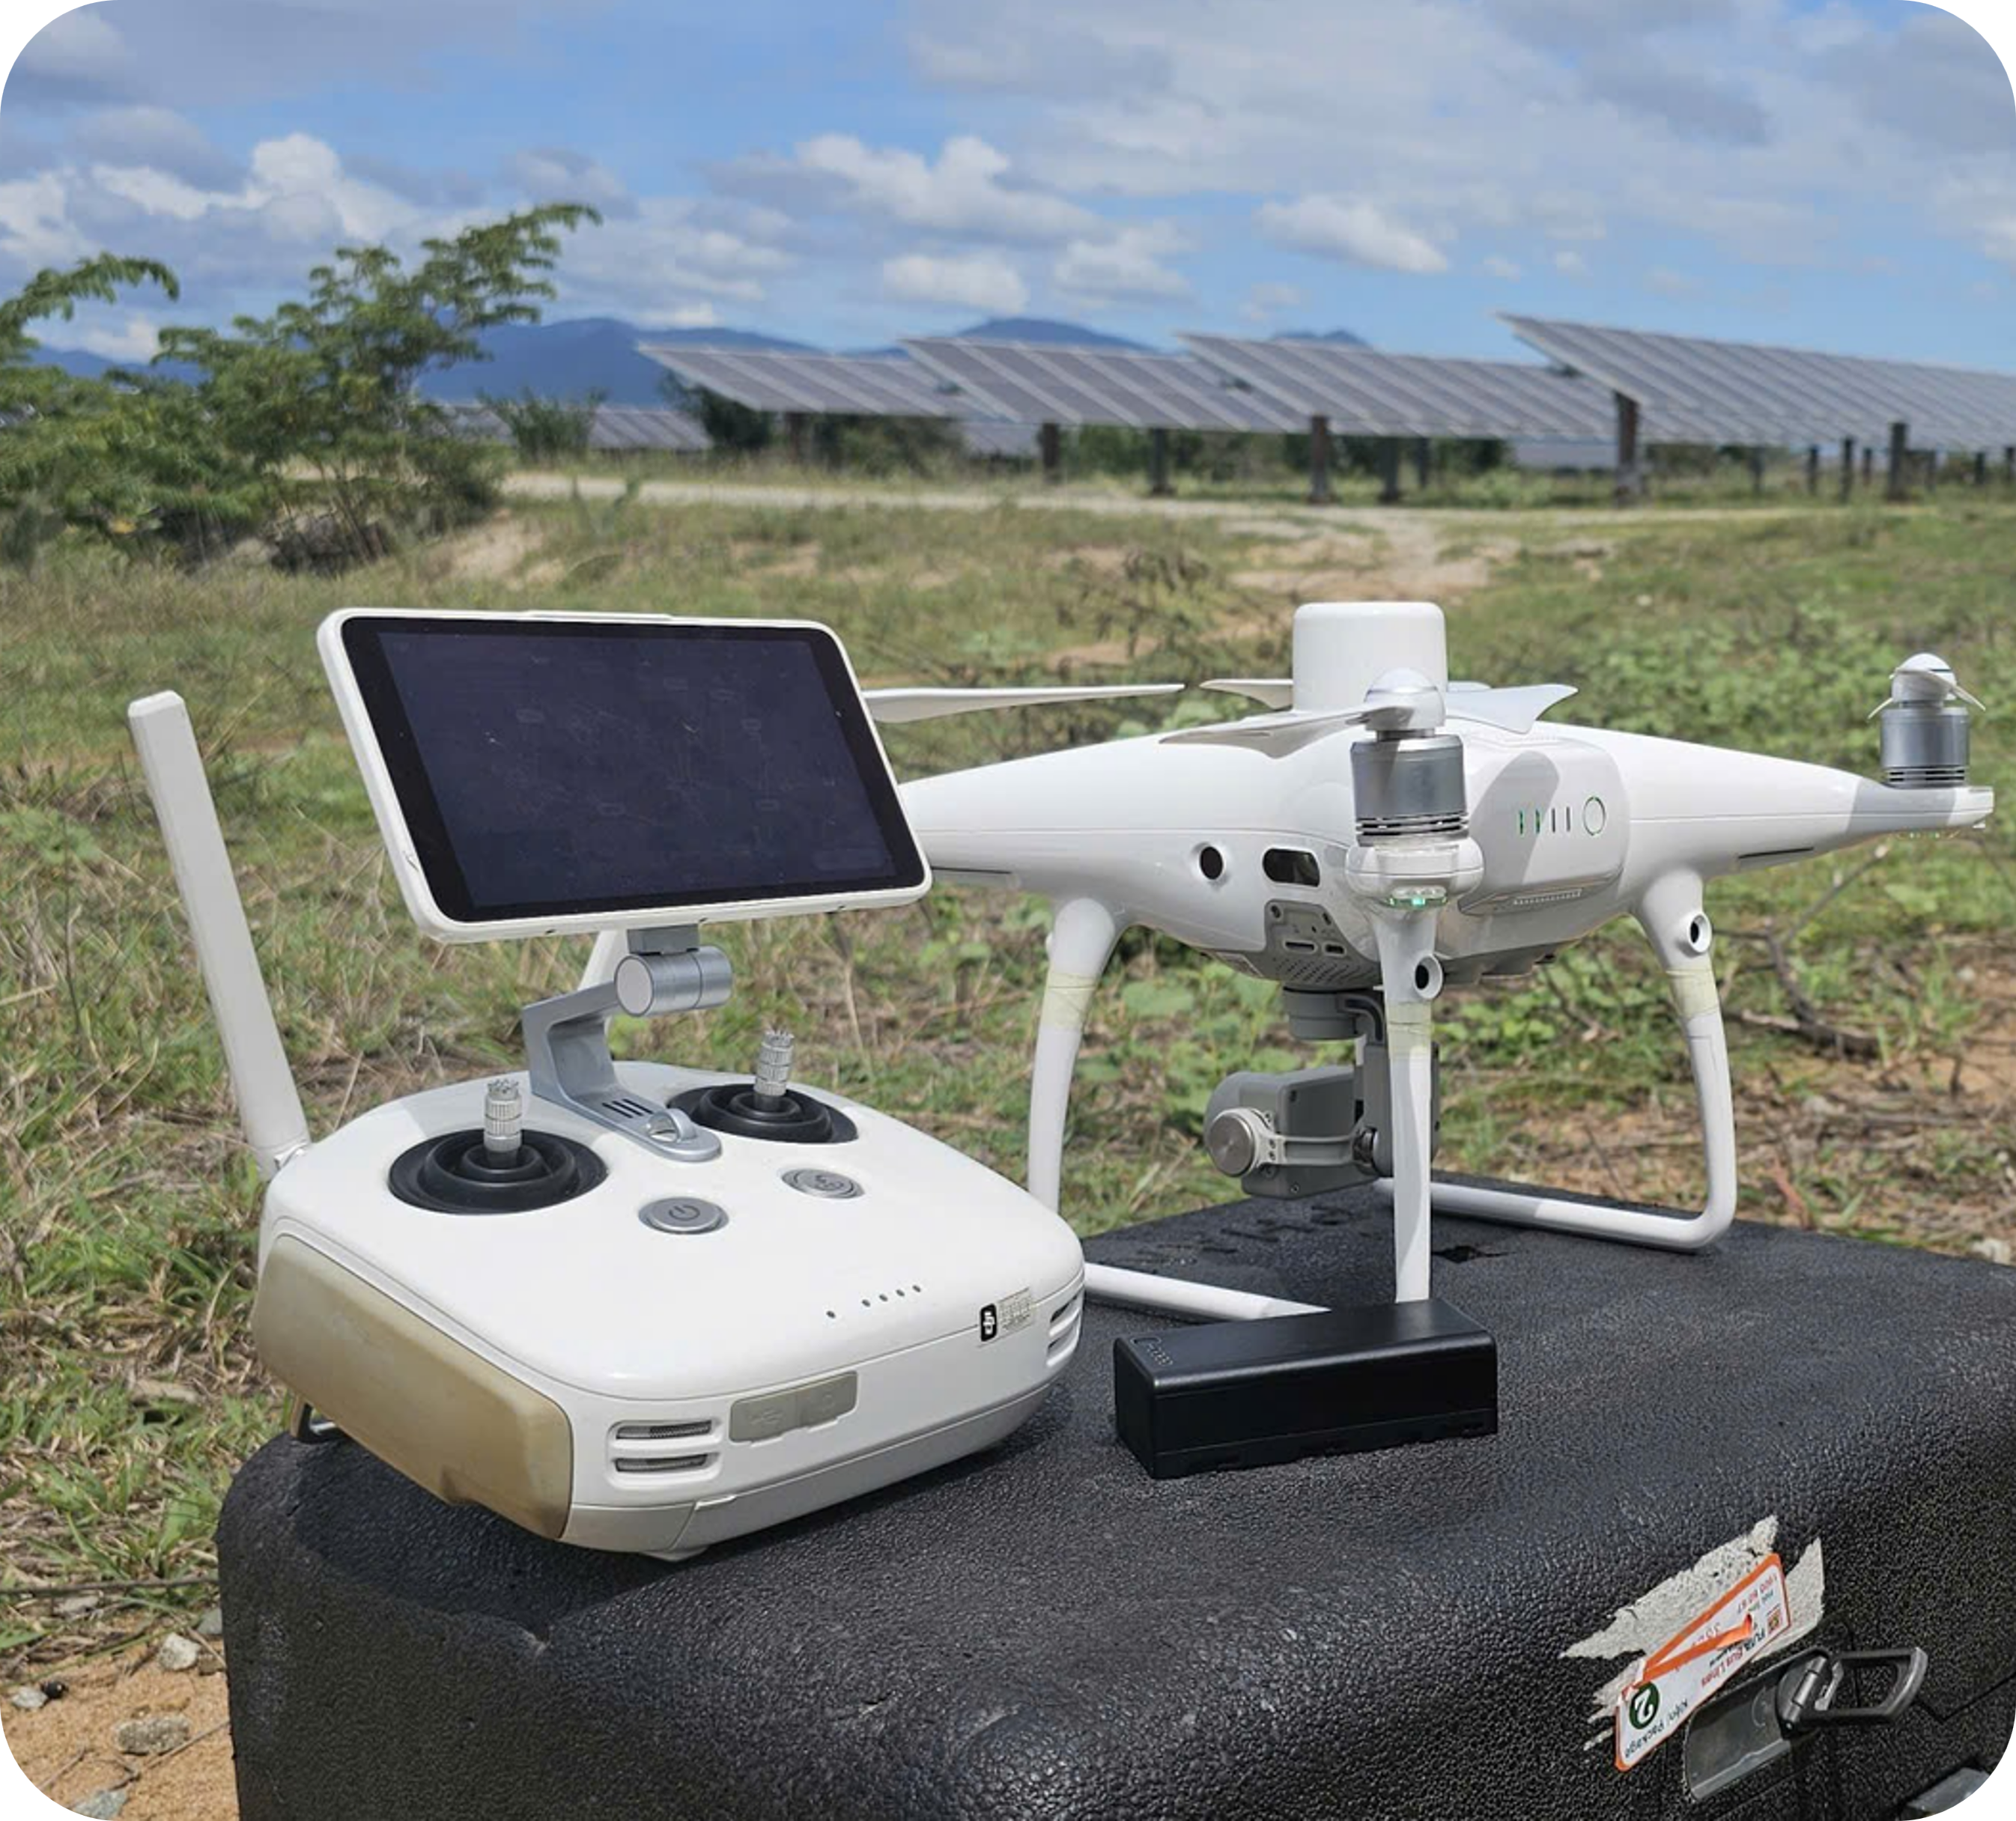
\includegraphics[width=\linewidth, keepaspectratio]{images/PhuongPhap/uav.png}};
            \end{tikzpicture}
        \end{column}
        
    \end{columns}
\end{frame}

\begin{frame}
\label{anhthuthapboiuav}
	\frametitle{ẢNH THU THẬP BỞI UAV}
	\begin{center}
		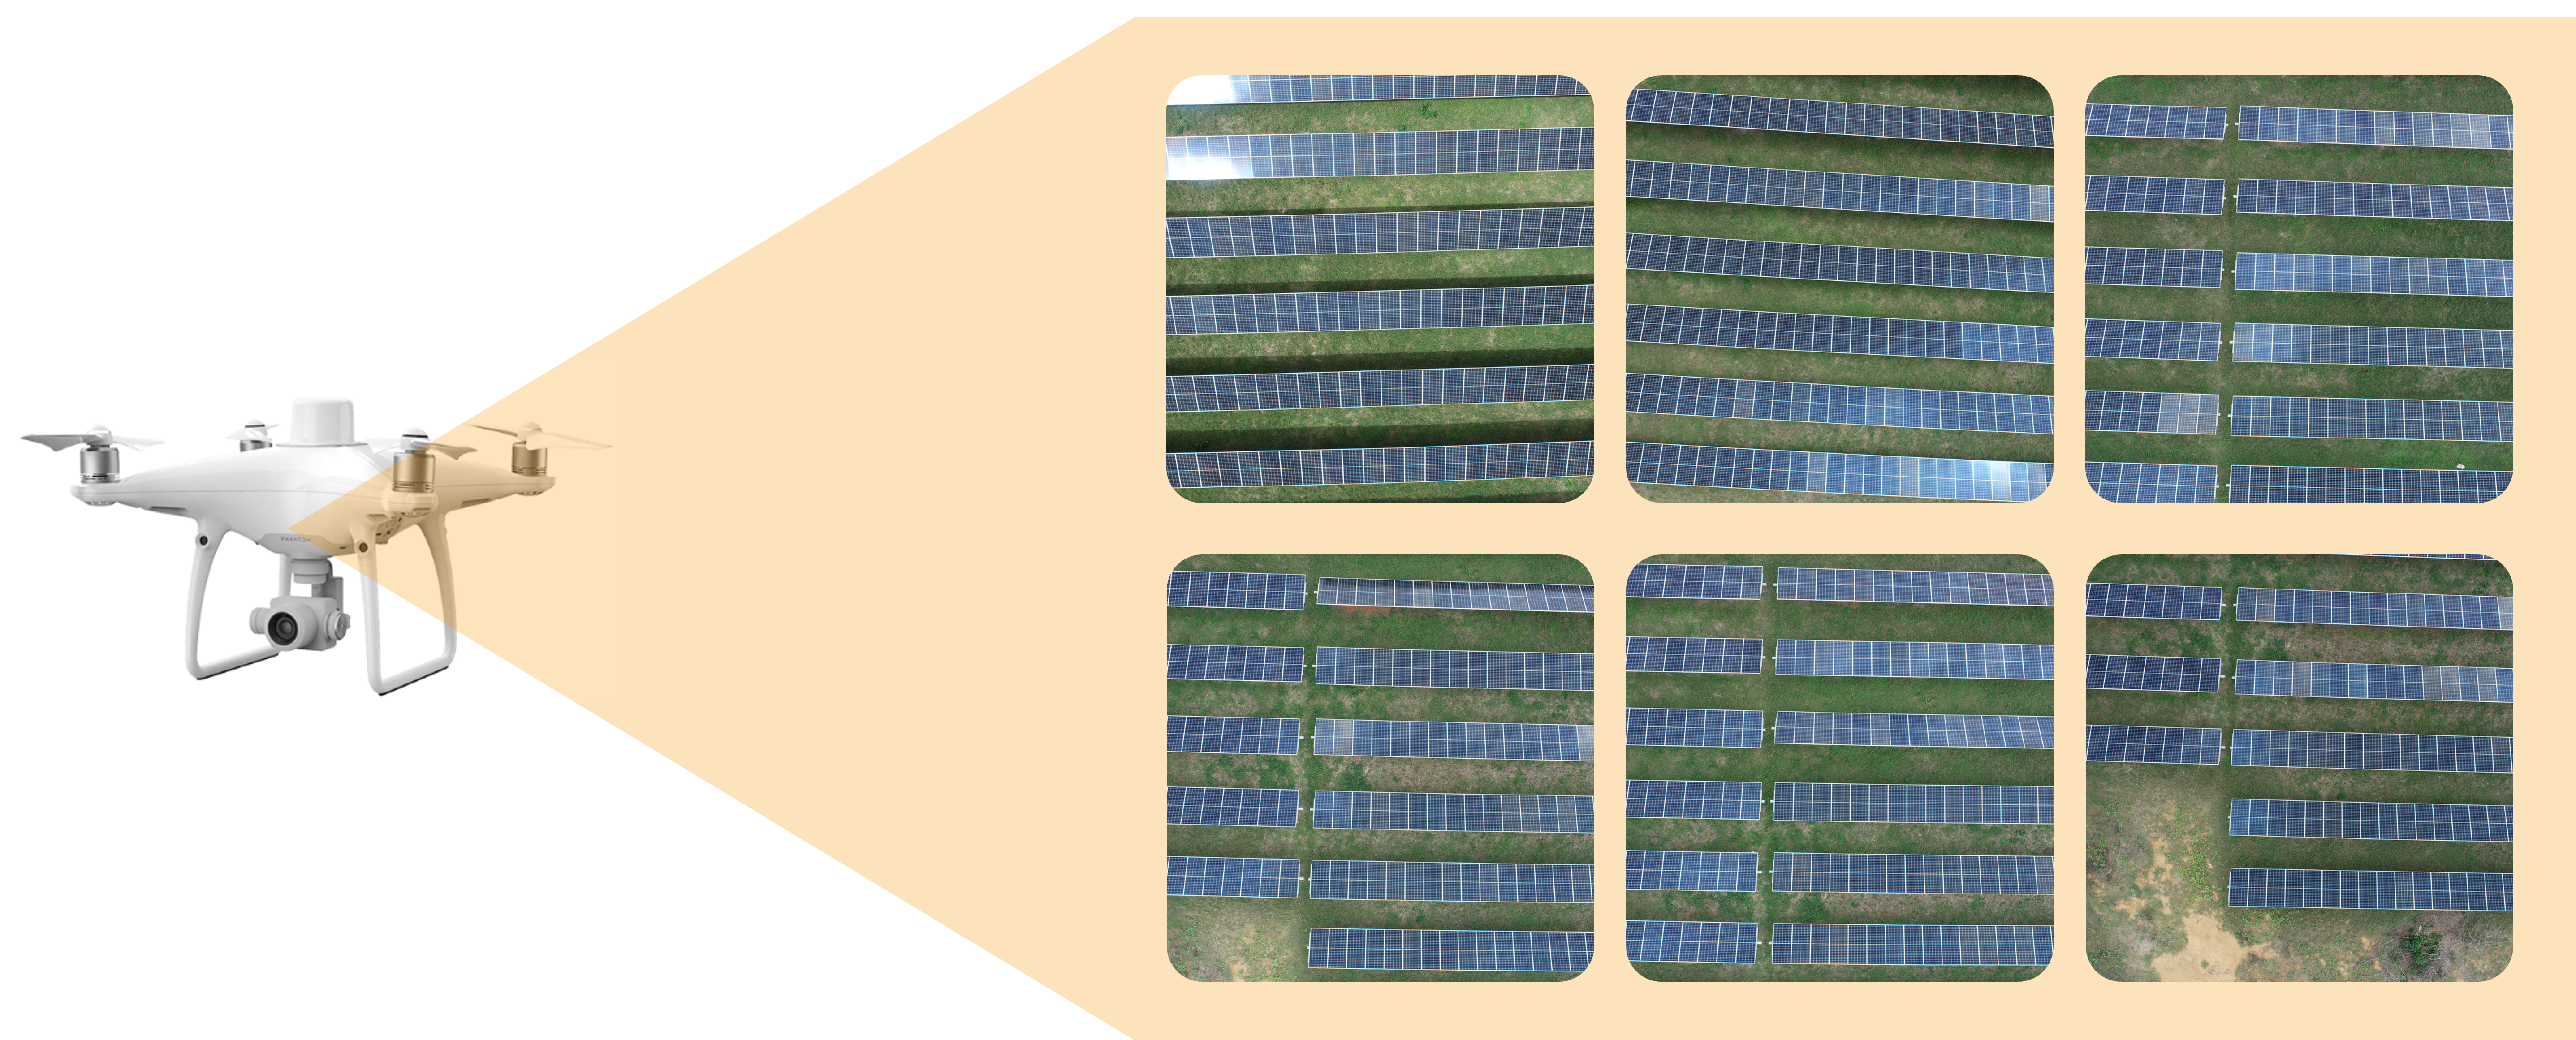
\includegraphics[width=0.8\textwidth]{images/PhuongPhap/thuthap.png}
	\end{center}
\end{frame}


\definecolor{myblue}{HTML}{0F52BA} % Màu xanh dương cho số liệu
\definecolor{mypinred}{HTML}{D93025} % Màu đỏ cho cái ghim
\definecolor{mybg}{HTML}{EFF1F3} % Màu xám nhạt nền box

\begin{frame}
    \frametitle{TÁCH CHIẾT TẤM PIN}
    
    \centering
    
    % Phần hình ảnh và nhãn đè lên (Overlay text)
    \begin{tikzpicture}
        % Chèn ảnh gốc, căn chỉnh độ rộng bằng chiều ngang văn bản
        % LƯU Ý: Thay đổi đường dẫn ảnh nếu cần thiết, LaTeX dùng dấu gạch chéo /
        \node[anchor=south west, inner sep=0] (image) at (0,0) {
            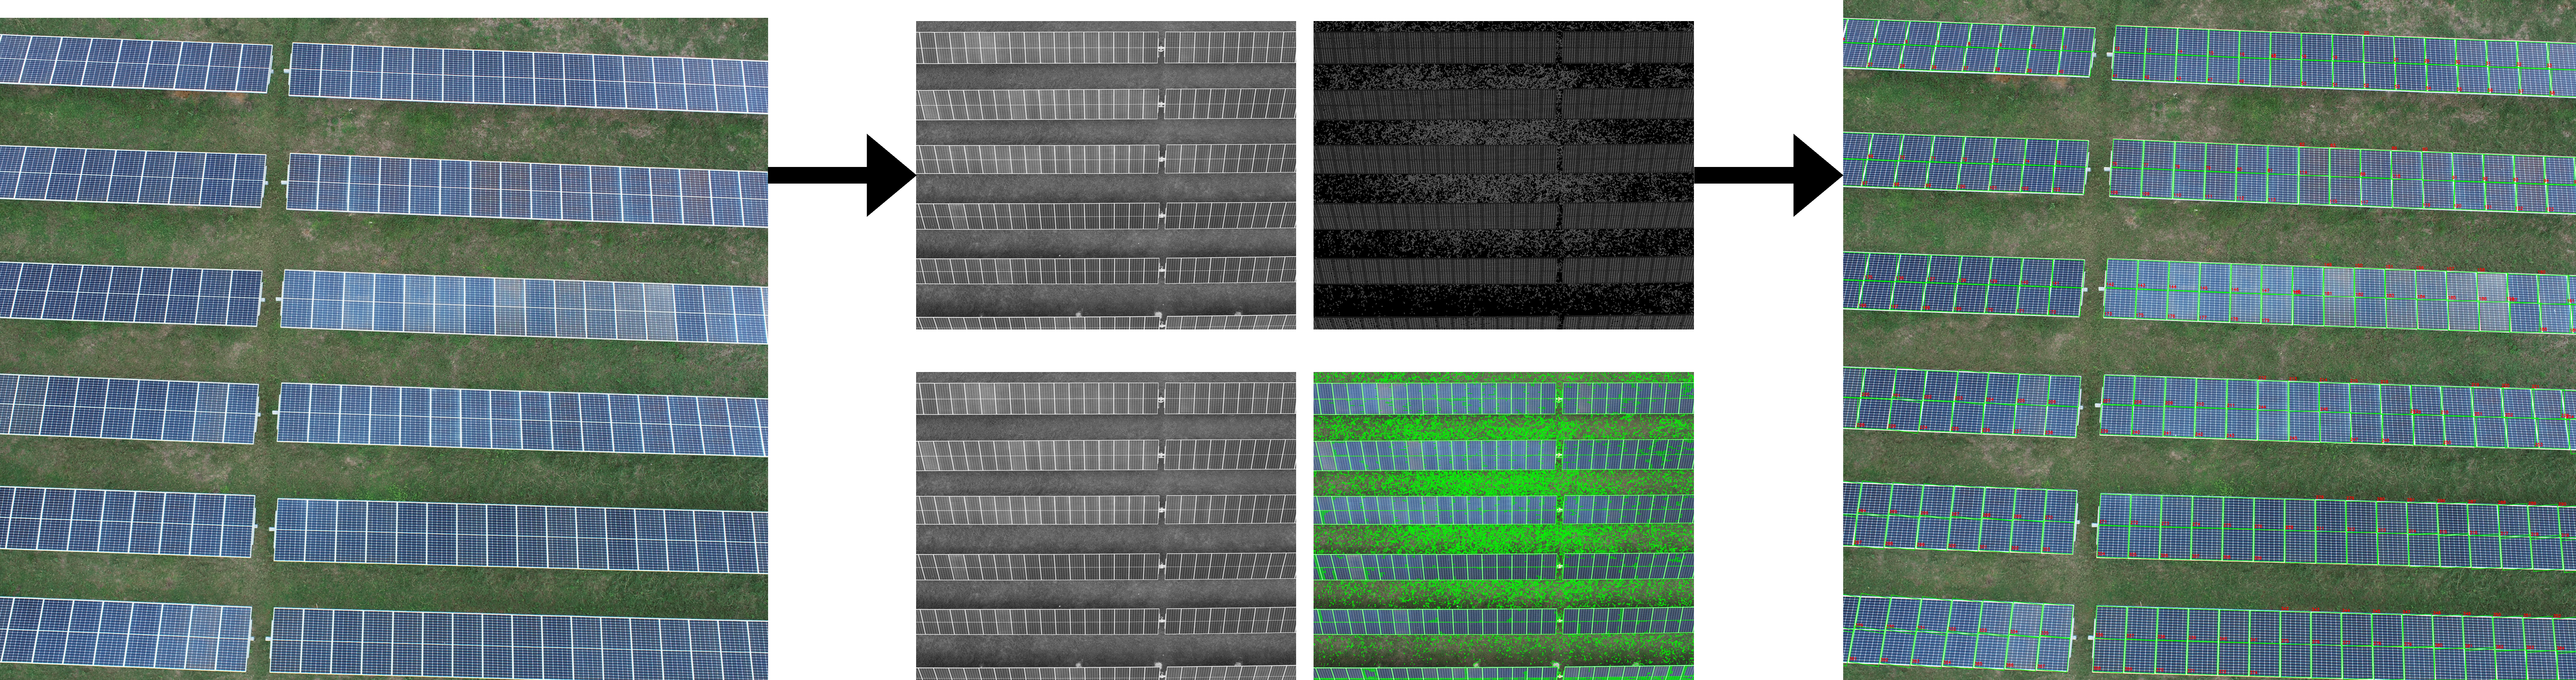
\includegraphics[width=\textwidth]{images/PhuongPhap/tachchiet.png}
        };
        
        % Tọa độ tương đối để đặt nhãn (cần tinh chỉnh nếu ảnh bị méo)
        % Quy ước: (0,0) là góc dưới trái ảnh, (1,1) là góc trên phải ảnh
\begin{scope}[x={(image.south east)}, y={(image.north west)}, font=\bfseries\tiny]
    
    % --- HÀNG TRÊN (Y khoảng 0.95) ---
    
    % Nhãn: Ảnh GRAY (Góc trên trái - Cột trái)
    % Dùng anchor=north west để chữ "treo" từ tọa độ xuống dưới
    \node[anchor=north west, text=white] at (0.37, 0.98) { 
        \textcolor{mypinred}{\faThumbtack}~Ảnh GRAY:
    };
    
    % Nhãn: Ảnh CANNY (Góc trên phải - Cột phải)
    % Tọa độ x bắt đầu từ 0.52 (qua nửa phải một chút)
    \node[anchor=north west, text=white] at (0.52, 0.98) { 
        \textcolor{mypinred}{\faThumbtack}~Ảnh CANNY:
    };
    
    % --- HÀNG DƯỚI (Y khoảng 0.48) ---
    
    % Nhãn: Ảnh BLUR (Góc dưới trái - Cột trái)
    % Đặt y=0.48 và anchor=north west để chữ nằm dưới đường kẻ giữa
    \node[anchor=north west, text=white] at (0.37, 0.48) { 
        \textcolor{mypinred}{\faThumbtack}~Ảnh BLUR:
    };
    
    % Nhãn: Ảnh CONTOUR (Góc dưới phải - Cột phải)
    \node[anchor=north west, text=white] at (0.52, 0.48) { 
        \textcolor{mypinred}{\faThumbtack}~Ảnh CONTOUR:
    };
    
\end{scope}
    \end{tikzpicture}
    
    \vspace{2pt} % Khoảng cách giữa ảnh và box bên dưới
    
    % Phần hộp nội dung kết quả (Box xám)
    \begin{tikzpicture}
        \node[
            fill=mybg, 
            rounded corners=5pt, 
            inner sep=8pt, 
            text width=0.95\textwidth, 
            anchor=north
        ] {
            \begin{columns}[T]
                % Cột tiêu đề trái
                \begin{column}{0.25\textwidth}
                    \textbf{Kết quả và\\độ tin cậy}
                \end{column}
                
                % Cột nội dung phải
                \begin{column}{0.75\textwidth}
                    \small
                    Quy trình đạt độ chính xác tách chiết \textbf{\textcolor{myblue}{96.9\%}} (Kiểm tra thủ công trên 1.000 mẫu)
                    
                    \vspace{0.3em} % Khoảng cách dòng
                    
                    Tự động trích xuất \textbf{\textcolor{myblue}{5.902}} ảnh tấm pin riêng lẻ từ 130 ảnh toàn cảnh.
                \end{column}
            \end{columns}
        };
    \end{tikzpicture}

\end{frame}

\begin{frame}
    \frametitle{TÁCH CHIẾT TẤM PIN}
    \vspace{0.2cm}

    % Chèn ảnh và chữ overlay
    \begin{figure}
        \centering
        \begin{tikzpicture}
            % 1. Chèn ảnh nền
            % Đảm bảo đường dẫn ảnh đúng với máy của bạn
            \node[anchor=south west, inner sep=0] (image) at (0,0) {
                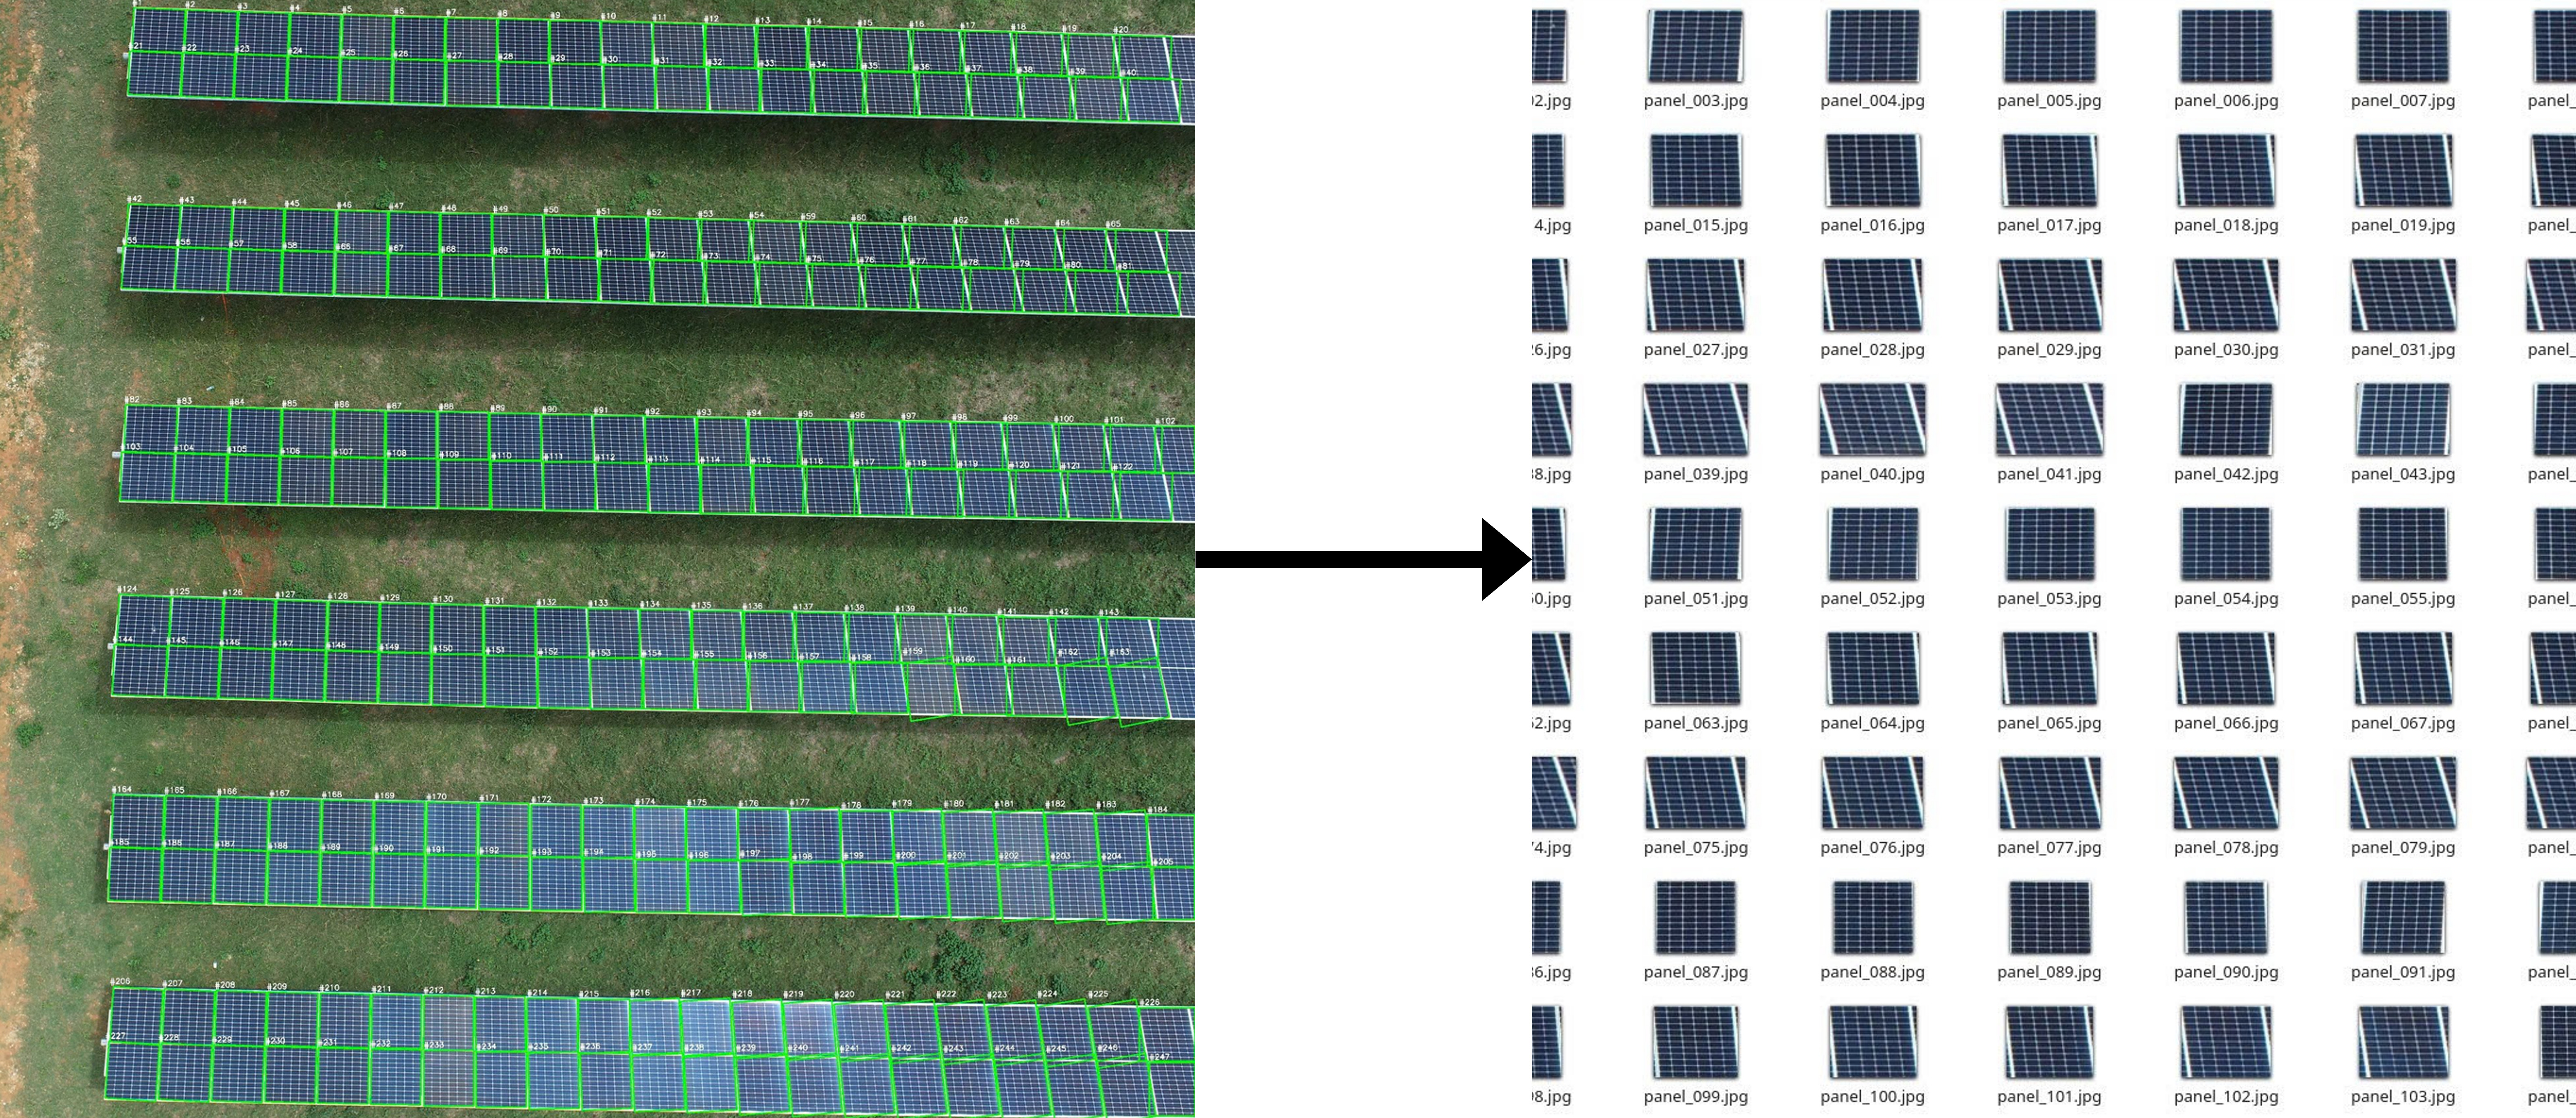
\includegraphics[width=\textwidth, height=0.6\textheight, keepaspectratio]{images/PhuongPhap/tachchietid.png}
            };

            % 2. Chèn chữ "ID tương ứng"
            % Sử dụng hệ tọa độ tương đối (0,0) đến (1,1) trên ảnh
            \begin{scope}[x={(image.south east)}, y={(image.north west)}]
                % - text=red: Màu đỏ
                % - font=\bfseries\small: Chữ in đậm và nhỏ lại (có thể dùng \footnotesize nếu muốn nhỏ hơn nữa)
                % - align=center: Căn giữa các dòng chữ
                % - at (0.5, 0.43): Đặt tại vị trí giữa theo chiều ngang (0.5) và bên dưới mũi tên theo chiều dọc (0.43)
                \node[text=red, font=\bfseries\tiny, align=center, anchor=north] at (0.53, 0.7) {ID\\tương ứng};
            \end{scope}
        \end{tikzpicture}
    \end{figure}

\end{frame}

% Định nghĩa màu sắc giống trong ảnh
\definecolor{customRed}{HTML}{FF3333} % Màu đỏ tươi cho số liệu
\definecolor{customGreen}{HTML}{2ECC71} % Màu xanh lá cho dấu check
\definecolor{customGray}{HTML}{CCCCCC} % Màu xám cho đường kẻ dọc

\begin{frame}
    \frametitle{BỘ DỮ LIỆU THỰC NGHIỆM}

    \vspace{0.5cm} % Căn chỉnh khoảng cách từ tiêu đề xuống nội dung

    \begin{columns}[T] % Căn lề trên (Top align) cho các cột
        
        % --- CỘT TRÁI (Số liệu tổng) ---
        \begin{column}{0.35\textwidth}
            \centering
            \vspace{0.5cm} % Đẩy nội dung xuống một chút cho cân giữa
            
            {\Large 130 ảnh UAV} \\[10pt]
            
            % Số to màu đỏ
            {\color{customRed}\textbf{\fontsize{45}{50}\selectfont 5.902}} \\[10pt]
            
            {\large Tổng số ảnh tấm pin}
        \end{column}

        % --- ĐƯỜNG KẺ DỌC ---
        \begin{column}{0.05\textwidth}
            \centering
            % Vẽ đường kẻ dọc màu xám
            {\color{customGray}\vrule width 1.5pt height 4.5cm}
        \end{column}

        % --- CỘT PHẢI (Chi tiết phân bố) ---
        \begin{column}{0.6\textwidth}
            \begin{itemize}
                \setlength\itemsep{1.5em} % Khoảng cách giữa các mục chính
                
                % Mục 1
                \item[\color{customGreen}\Huge\checkmark] 
                    {\large \textbf{Phân bố nhãn:} 3.047 Bình thường / 2.854 Lỗi}
                
                % Mục 2
                \item[\color{customGreen}\Huge\checkmark] 
                    {\large \textbf{Chia tập dữ liệu:}}
                    \vspace{0.3cm}
                    \begin{itemize}
                        \setlength\itemsep{0.5em} % Khoảng cách các mục con
                        \normalsize
                        \item Training: 70\% - 4.131 (Học mô hình)
                        \item Validation: 15\% - 885 (Tinh chỉnh siêu tham số)
                        \item Test: 15\% - 886 (Đánh giá cuối cùng)
                    \end{itemize}
            \end{itemize}
        \end{column}
        
    \end{columns}
\end{frame}


\begin{frame}
    \frametitle{TĂNG CƯỜNG DỮ LIỆU}
    \centering
    
    % Thiết lập chiều rộng của cột (gần một nửa slide trừ đi khoảng đệm)
    \newcommand{\colW}{0.46\textwidth}
    % Thiết lập CHIỀU CAO CỐ ĐỊNH cho mỗi ô (QUAN TRỌNG ĐỂ KHÔNG BỊ DÃN)
    \newcommand{\rowH}{3.2cm} 
    % Thiết lập chiều cao ảnh tối đa
    \newcommand{\imgH}{2.0cm}

    % Bắt đầu bảng với các đường kẻ | ở giữa
    \begin{tabular}{c|c}
    
        % --- GÓC TRÊN TRÁI ---
        \begin{minipage}[c][\rowH][c]{\colW}
            \centering
            \textbf{Xoay (Rotation): +/- 15$^\circ$} \\ 
            \vspace{2pt} % Khoảng cách rất nhỏ
            \includegraphics[height=\imgH, keepaspectratio]{images/PhuongPhap/dataaugment/rotation.png}
        \end{minipage}
        & 
        % --- GÓC TRÊN PHẢI ---
        \begin{minipage}[c][\rowH][c]{\colW}
            \centering
            \textbf{Lật (Flip): Ngang/Dọc} \\ 
            \vspace{2pt}
            \includegraphics[height=\imgH, keepaspectratio]{images/PhuongPhap/dataaugment/flip.png}
        \end{minipage}
        \\ 
        \hline % ĐƯỜNG KẺ NGANG LIỀN MẠCH
        
        % --- GÓC DƯỚI TRÁI ---
        \begin{minipage}[c][\rowH][c]{\colW}
            \centering
            \vspace{2pt} % Đẩy nhẹ nội dung xuống khỏi đường kẻ
            \textbf{Color Jitter: Độ Sáng/Tương Phản} \\ 
            \vspace{2pt}
            \includegraphics[height=\imgH, keepaspectratio]{images/PhuongPhap/dataaugment/color.png}
        \end{minipage}
        & 
        % --- GÓC DƯỚI PHẢI ---
        \begin{minipage}[c][\rowH][c]{\colW}
            \centering
            \vspace{2pt}
            \textbf{Noise Injection: Nhiễu Gaussian} \\ 
            \vspace{2pt}
            \includegraphics[height=\imgH, keepaspectratio]{images/PhuongPhap/dataaugment/noise.png}
        \end{minipage}
        
    \end{tabular}
\end{frame}

% --- MÀU SẮC ---
\definecolor{myBlueLine}{HTML}{0072BC}
\definecolor{myBlueBack}{HTML}{F0F6FA}
\definecolor{myOrangeLine}{HTML}{F7941D}
\definecolor{myOrangeBack}{HTML}{FFF9F0}

% --- STYLE KHUNG (Đã thu gọn padding) ---
\tcbset{
    myboxstyle/.style={
        enhanced,
        boxrule=0pt,
        leftrule=0pt,
        arc=3pt,
        auto outer arc,
        % GIẢM PADDING ĐỂ TIẾT KIỆM CHỖ
        left=6pt, right=6pt, top=5pt, bottom=5pt, 
        boxsep=0pt,
    }
}

% Thêm tùy chọn [shrink] để Beamer tự động co nhỏ nếu vẫn bị tràn
\begin{frame} 
    \frametitle{CHIẾN LƯỢC HUẤN LUYỆN}

    \vspace{-0.2cm} 

    % --- KHỐI DỮ LIỆU (TRÊN) ---
    \begin{tcolorbox}[
        myboxstyle,
        colback=myBlueBack,
        colframe=myBlueLine,
        width=\textwidth
    ]
        \small 
        \begin{center}
            \textbf{Dữ Liệu}
        \end{center}
        \vspace{-8pt} % Kéo nội dung sát tiêu đề hơn
        
        \begin{itemize}
            \setlength\itemsep{0pt}
            \item \textbf{Tổng:} 5,902 ảnh.
            \item \textbf{Phân chia:} Train 70\% -- Val 15\% -- Test 15\%.
            \item \textbf{Nhãn:} Normal / Defect.
        \end{itemize}
    \end{tcolorbox}
    
    \vspace{0.2cm} % Khoảng cách giữa 2 khối

    % --- KHỐI KỸ THUẬT (DƯỚI) ---
    \begin{tcolorbox}[
        myboxstyle,
        colback=myOrangeBack,
        colframe=myOrangeLine,
        width=\textwidth
    ]
        \small 
        \begin{center}
            \textbf{Kỹ Thuật}
        \end{center}
        \vspace{-8pt}

        \begin{itemize}
            \setlength\itemsep{2pt} 
            \item \textbf{Augmentation:} Xoay, Lật, Chỉnh màu, Nhiễu Gaussian.
            \item \textbf{Optimizer:} Adam (LR $1e-4$).
            \item \textbf{Early Stopping:} Patience = 5.
            \item \textbf{Loss:} Weighted Cross-Entropy \& Focal Loss.
        \end{itemize}
    \end{tcolorbox}

\end{frame}
